%% RiSE Latex Template - version 0.5
%%
%% RiSE's latex template for thesis and dissertations
%% http://risetemplate.sourceforge.net
%%
%% (c) 2012 Yguaratã Cerqueira Cavalcanti (yguarata@gmail.com)
%%          Vinicius Cardoso Garcia (vcg@cin.ufpe.br)
%%
%% This document was initially based on UFPEThesis template, from Paulo Gustavo
%% S. Fonseca.
%%
%% ACKNOWLEDGEMENTS
%%
%% We would like to thanks the RiSE's researchers community, the 
%% students from Federal University of Pernambuco, and other users that have
%% been contributing to this projects with comments and patches.
%%
%% GENERAL INSTRUCTIONS
%%
%% We strongly recommend you to compile your documents using pdflatex command.
%% It is also recommend use the texlipse plugin for Eclipse to edit your documents.
%%
%% Options for \documentclass command:
%%         * Idiom
%%           pt   - Portguese (default)
%%           en   - English
%%
%%         * Text type
%%           bsc  - B.Sc. Thesis
%%           msc  - M.Sc. Thesis (default)
%%           qual - PHD qualification (not tested yet)
%%           prop - PHD proposal (not tested yet)
%%           phd  - PHD thesis
%%
%%         * Media
%%           scr  - to eletronic version (PDF) / see the users guide
%%
%%         * Pagination
%%           oneside - unique face press
%%           twoside - two faces press
%%
%%		   * Line spacing
%%           singlespacing  - the same as using \linespread{1}
%%           onehalfspacing - the same as using \linespread{1.3}
%%           doublespacing  - the same as using \linespread{1.6}
%%
%% Reference commands. Use the following commands to make references in your
%% text:
%%          \figref  -- for Figure reference
%%          \tabref  -- for Table reference
%%          \eqnref  -- for equation reference
%%          \chapref -- for chapter reference
%%          \secref  -- for section reference
%%          \appref  -- for appendix reference
%%          \axiref  -- for axiom reference
%%          \conjref -- for conjecture reference
%%          \defref  -- for definition reference
%%          \lemref  -- for lemma reference
%%          \theoref -- for theorem reference
%%          \corref  -- for corollary reference
%%          \propref -- for proprosition reference
%%          \pgref   -- for page reference
%%
%%          Example: See \chapref{chap:introduction}. It will produce 
%%                   'See Chapter 1', in case of English language.
%%
%% Citation commands:
%%          \citet (from natbib) -- To cite a reference as part of the narrative
%%          \citep (from natbib) -- To cite a reference between parenthesis
%%          citationblock environment -- To produce direct citation blocks according to the ABNT

\documentclass[pt,oneside,onehalfspacing,bscprop]{risethesis}
\usepackage{colortbl}
\usepackage{color}
\usepackage[table,xcdraw]{xcolor}
\usepackage{longtable}
\usepackage{microtype}
\usepackage{bibentry}
\usepackage{subfig}
\usepackage{multirow}
\usepackage{multicol}
\usepackage{rotating}
\usepackage{booktabs}
\usepackage{pdfpages}
\usepackage{caption}
\usepackage{lipsum}
\usepackage{sectsty}
\usepackage{listings}

\definecolor{dkgreen}{rgb}{0,0.6,0}
\definecolor{gray}{rgb}{0.5,0.5,0.5}
\definecolor{mauve}{rgb}{0.58,0,0.82}

\lstset{frame=tb,
  language=C++,
  aboveskip=3mm,
  belowskip=3mm,
  showstringspaces=false,
  columns=flexible,
  basicstyle={\small\ttfamily},
  numbers=none,
  numberstyle=\tiny\color{gray},
  keywordstyle=\color{blue},
  commentstyle=\color{dkgreen},
  stringstyle=\color{mauve},
  breaklines=true,
  breakatwhitespace=true,
  tabsize=3
}
\usepackage{tikz}
\usetikzlibrary{calc,trees,positioning,arrows,chains,shapes.geometric,%
    decorations.pathreplacing,decorations.pathmorphing,shapes,%
    matrix,shapes.symbols}
\tikzset{
>=stealth',
  punktchain/.style={
    rectangle, 
    rounded corners, 
    % fill=black!10,
    draw=black, very thick,
    text width=7em, 
    minimum height=3em, 
    text centered, 
    on chain},
  line/.style={draw, thick, <-},
  element/.style={
    tape,
    top color=white,
    bottom color=blue!50!black!60!,
    minimum width=8em,
    draw=blue!40!black!90, very thick,
    text width=10em, 
    minimum height=3.5em, 
    text centered, 
    on chain},
  every join/.style={->, thick,shorten >=1pt},
  decoration={brace},
  tuborg/.style={decorate},
  tubnode/.style={midway, right=2pt},
}

\captionsetup[table]{position=top,justification=centering,width=.85\textwidth,labelfont=bf,font=footnotesize}
\captionsetup[lstlisting]{position=top,justification=centering,width=.85\textwidth,labelfont=bf,font=footnotesize}
\captionsetup[figure]{position=bottom,justification=centering,width=.85\textwidth,labelfont=bf,font=footnotesize}

%% Chapter and (Sub)Section fonts must be same size as text (12)
\sectionfont{\fontsize{12}{15}\selectfont}
\subsectionfont{\fontsize{12}{15}\selectfont}
\subsubsectionfont{\fontsize{12}{15}\selectfont}

%% Change the following pdf author attribute name to your name.
\usepackage[linkcolor=black,
            citecolor=black,
            urlcolor=black,
            colorlinks,
            pdfpagelabels,
            pdftitle={Rise Thesis Template (ABNT)},
            pdfauthor={Rise Thesis Template (ABNT)},
            breaklinks=true]{hyperref}

\address{RECIFE}

\universitypt{Universidade Federal de Pernambuco}
\universityen{Federal University of Pernambuco}

\departmentpt{Centro de Informática}
\departmenten{Center for Informatics}

\programpt{Graduação em Engenharia da computaç}
\programen{Undergraduate in Computer Engineering}

\majorfieldpt{Engenharia da computação}
\majorfielden{Computer Engineering}

\title{Evaluating Reinforcement Learning on Robocup Soccer Simulation 2D}

\date{2019}

\author{Mateus Gonçalves Machado}
\adviser{Tsang Ing Ren}

% Macros (defines your own macros here, if needed)
\def\x{\checkmark}

\begin{document}

\frontmatter

\frontpage

%\presentationpage

%\begin{dedicatory}
%I dedicate this thesis to all my family, friends and professors who gave me the
%necessary support to get here.
%\end{dedicatory}

%\acknowledgements
%Gostaria de agradecer primeiramente a minha família por ter me dado sempre uma educação incrível. Dona Selma, seu Alexandre, parabéns por estarem formando o último filho. Agradecer a meu irmão e irmã que sem eles eu tenho certeza que não teria tanta inspiração para a maioria das coisas da minha vida inteira. Gostaria também de agradecer à Samara, minha namorada, que por querer ter tanta força e garra como ela, venho me tornando melhor a cada dia. Agradecer aos meus amigos principalmente (só pela ordem alfabética): Ana Luiza, Anna Letícia, Cristiano Oliveira e Jailson Gomes. Obrigado por estarem sempre e sempre comigo, tenham certeza que tenho em vocês irmãos que escolhi ter. Um obrigado especialsíssimo a Walber Macêdo por ter limite emocional para me aguentar.
E claro, obrigado a equipe que se tornou minha segunda família, a principal razão de eu ter seguido essa linha de pesquisa. Obrigado RobôCIn! A cada um que agradeço neste documento, amo vocês demais.


\begin{center}
MAMÃE ACABOU!
\end{center}


\let\cleardoublepage\clearpage

\resumo
% Escreva seu resumo no arquivo resumo.tex
{\parindent0pt
	A liga de simulação 2D de futebol do RoboCup é uma das mais maduras da competição, iniciada em 1996. Aprendizagem supervisionada e algoritmos determinísticos são as técnicas mais usadas pelas 5 melhores equipes. Pesquisas recentes usando Aprendizagem Profunda por Reforço (APR) para treinar agentes autônomos em sistemas multiagentes superaram os agentes com base em algoritmos supervisionados ou determinísticos. Um exemplo é a equipe CYRUS2019 produziu jogadores defensivos treinados com o APR, alcançando em terceiro lugar na RoboCup 2019. Este trabalho pretende comparar três técnicas de APR em agentes defensivos com base no CYRUS2019, adaptando o \textit{Half Field Offensive} para ser um ambiente semelhante aos da OpenAI GYM e aplicar a melhor técnica aos agentes do time RoboCIn2d.
}

\abstract
% Write your abstract in a file called abstract.tex
{\parindent0pt
	The Simulation 2D Football league of RoboCup is one of the most matures leagues of the competition having started in 1996. Supervised Learning and deterministic algorithms are the usual techniques used by the TOP 5 teams. Recent researches using Deep Reinforcement Learning to train autonomous agents in multi-agent systems have shown that it outperforms agents based on supervised or deterministic algorithms. The team CYRUS2019 has released defensive players trained with Deep Reinforcement Learning achieving in third place on RoboCup2019. This work intents to compare three DRL techniques for defensive agents based on CYRUS2019 adapting the Half Field Offensive environment to an OpenAI GYM like environment and apply the best technique on RoboCIn2d's agents.
}

% List of figures
% \listoffigures

% List of tables
% \listoftables

% List of acronyms
% Acronyms manual: http://linorg.usp.br/CTAN/macros/latex/contrib/acronym/acronym.pdf
% \listofacronyms
% \begin{acronym}[ACRONYM] 
% Change the word ACRONYM above to change the acronym column width.
% The column width is equals to the width of the word that you put.
% Read the manual about acronym package for more examples:
%   http://linorg.usp.br/CTAN/macros/latex/contrib/acronym/acronym.pdf

\end{acronym}

% Summary (tables of contents)
% \tableofcontents

\mainmatter

% Uncomment to graduation
% \chapter{Introduction}
A liga de Simulação de Futebol 2D da \cite{robocup} (Sim2d) é uma das mais antigas da competição, tendo início em 1996. As técnicas mais usadas nos 5 melhores times da liga são Aprendizagem Supervisionada e Algorítmos determinísticos. Pesquisas recentes  tem mostrado que usar Aprendizagem Profunda por Reforço (APR) para treinar agentes autônomos em sistemas multi agentes se obtém uma performance maior. O time CYRUS2019, \cite{cyrus}, fez sua linha defensiva de jogadores usando APR e conquistou o terceiro lugar na RoboCup2019.Este trabalho pretende incluir uma linha de defesa treinada com uma técnica de APR baseado no time CYRUS2019, adpatando o ambiente do \textit{Half Field Offensive} para um ambiente OpenAI GYM, \cite{gym}, e aplicar ao time da equipe \cite{robocin}.

Com o objetivo de vencer o time capeão mundial humano de 2050, a RoboCup tem sido uma grande competição para desenvolver e compartilhar técnicas sobre robótica e agentes autônomos. Entre as ligas, Simulação de Futebol 2D é um dos melhores ambientes para se aplicar algoritmos de aprend
With the goal of beating the human soccer World Champion team in 2050, Robocup has been a great competition to develop and share robotics and autonomous agents techniques. Among the leagues, Soccer Simulation 2D league is a great domain to invest machine learning (ML) algorithms and it is been a challenge as \cite{RoboCupAIChallenge} say. At the very beginning of the league at 1996, the competitors used to implement by their own hands the behaviours of the players. Once it's a simulated league, Machine Learning techniques became natural since there is no mechanic or electronic interference. The German team, Brainstormers was one of the pilots with an approach using Reinforcement Learning (\cite{brainstormers2002}). Since then teams frequently uses Artificial Intelligence algorithms to have unnatural and unpredictable behaviours. 

This work focus on the defense line, specifically in a single intelligent defender cooperating with a hand-coded goalie against a single attacker. As there is more works about the attackers like \cite{passingCrit}, \cite{keepawayRL} and more recent \cite{hausknecht2015deep}, the defense line became attractive to the RoboCIn team.

\cite{deepmind} researchers \cite{dqn} have shown that Deep Q Learning was so effective on Atari games that it outplays human controlled agents. In 2015 Deepmind's AlphaGo agent, \cite{alphago}, won from the European Go Champion Fan Hui and later on 2016 from Lee Sedol, one of the best worldwide. Since then OpenAI and DeepMind has invested a lot of effort on Reinforcement Learning (RL) and Autonomous Agents (AA) systems. Recently \cite{openai5} has become the best agent on \cite{dota2} on 1v1 games and it has a great teamwork performance on 5v5 games winning from most of amateur teams and a few professionals.

Inspired by those recent researches \cite{cyrus} modeled a defensive autonomous agent and it has almost the same efficiency of the champions' Fractals (\cite{glidersv2}, and Helios, \cite{helios2016}, defenses. Based on \cite{cyrus} work we will compare three Deep Reinforcement Learning models, \cite{dqn}, \cite{DDQN}, \cite{DDPG}, applied to an environment very likely to the real Soccer Simulation 2D.

% \chapter{Background}\label{chapter:background}
In this chapter we introduce techniques described in Team Description Papers of the \cite{robocup} and papers about Soccer Simulation 2D. In Section \ref{section:DefensiveDeterministic} we present deterministic techniques for defensive agents. Also in this chapter, in Section \ref{section:RLAgents} we show Reinforcement Learning techniques applied to defensive.

\section{Deterministic Agents}\label{section:DefensiveDeterministic}
In this section we shall explain some successful deterministic techniques applied to Soccer Simulation 2D league. Most of them are very useful as baseline or the teams actual defense line.

\subsection{Marlik2011 Defense}
\cite{marlik2011} created one of the best Defensive behaviour presented in the Soccer Simulation 2D League used since then in great teams like Fractals2019, \cite{glidersv2}. It was combined by three high-level actions: Cross Mark, Play\_on Mark and Block. Since they released the code, the RoboCIn team included those actions to their agent and it raised up to 60\% of the successful defenses.

\subsubsection{Cross Mark}
This behaviour occurs when an opponent reaches near one of the defensive corner flags, usually when -36 > Ball-X > -53 and 20 < |Ball-Y| < 34. The main idea of the algorithm is to position the marker between the nearest attacker and the ball to reach the ball faster. When the number of defenders is greater than the attackers, man-to-man marking will be done and the rest of the markers will guard the goal for probable shots. When attackers have an advantage, the three midfielders (usually numbers 6, 7 and 8) will try to mark opponents depending on their stamina. In Figure \ref{fig:crossmark} we can see an example of the behaviour.

\begin{figure}[H]
    \centering
    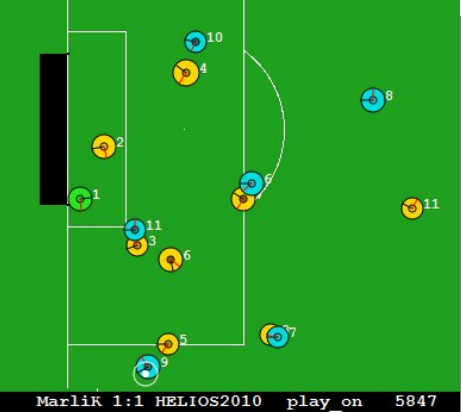
\includegraphics[scale=0.5]{images/cross_mark.png}
    \caption{Cross Mark behaviour. Observe the positioning of numbers 3, 4, 7 and 8 how the get in "front" of the attackers. Image from \cite{marlik2011}.}
    \label{fig:crossmark}
\end{figure}


\subsubsection{Play\_on Mark}
This type of marking is to avoid through passes and it is only applied on defenders, usually numbers 2, 3, 4 and 5. The idea is to disarm the attack when they are trying to break the defense line. Depending on attackers position and the defenders formation, the marker will choose one of the attackers to stay "behind" and then block a possible through pass. In Figure \ref{fig:playonmark} and \ref{fig:playonmark2} we can see examples of the behaviour.

\begin{figure}[H]
    \centering
    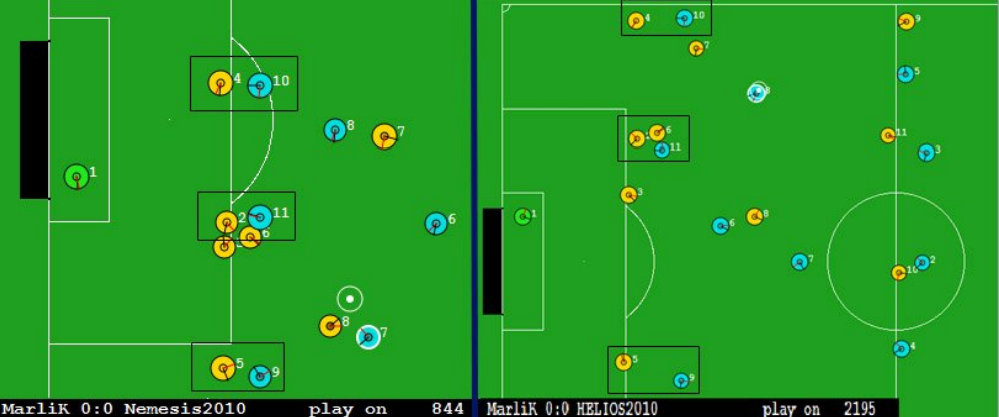
\includegraphics[scale=0.5]{images/play_on_mark.png}
    \caption{Play\_on Mark behaviour. Image from \cite{marlik2011}.}
    \label{fig:playonmark}
\end{figure}

\begin{figure}[H]
    \centering
    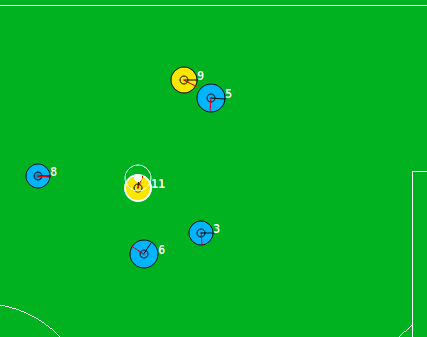
\includegraphics[scale=0.5]{images/play_on_mark2.png}
    \caption{Play\_on Mark behaviour. Observe the positioning of numbers 5 and 3 ready to block a through pass.}
    \label{fig:playonmark2}
\end{figure}

\subsubsection{Block}
Block is the most efficient technique of Marlik2011. Including only it in RoboCIn's code, the behaviour reduced from an average of 7 goals taken from  HELIOS2018 to an average of 2 goals taken. 

It has two important parts: moving to the best block point and decide how to act then. When the defender is the near from the ball, the best block point is calculated by a prediction of opponent's future dribble target. When the agent is too far from the attacker in possession, it marks the nearest opponent, see Figure \ref{fig:block}. Once the agent have reached the best position to block the attack, the defender will decide if it will continue doing the block, intercept the ball or push the attackers back, see Figure \ref{fig:block2}.

\begin{figure}[h]
    \centering
    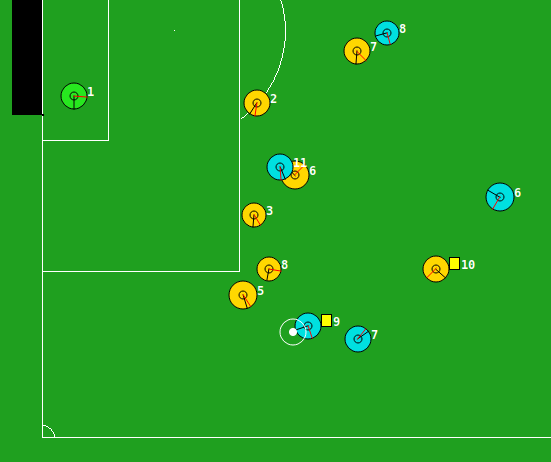
\includegraphics[scale=0.5]{images/block_pass.png}
    \caption{Block behaviour. Observe the yellow team positioning of numbers 6, 7 and 10 ready to block the pass.}
    \label{fig:block}
\end{figure}

\begin{figure}[H]
    \centering
    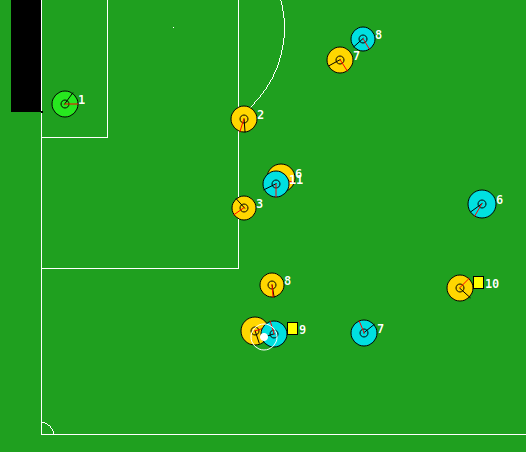
\includegraphics[scale=0.5]{images/marlik_block.png}
    \caption{Block behaviour. Observe the positioning of number 5 going to intercept the ball.}
    \label{fig:block2}
\end{figure}


\subsection{WrightEagle2014 Defense}
The WrightEagle team, \cite{wrighteagle2014}, did an interesting research on defenses areas and ranges. Their algorithm draws defensible areas based on defender formation's position and a number K opponents attackers. K represents how many opponents can represent better the attack or the most valuated weights calculated by the algorithm. The K weights are summed up and normalized and then the area with greater weight is chosen to be defended. In figure \ref{fig:defensenet} we can see an example of defense nets.

\subsection{Gliders2d Defense}
\cite{glidersv1} showed a simple defense improving with Gliders2D that caused their winning of RoboCup 2016. They fine tuned the pressing variable considering the role of the agent, the position of the ball and the opponent team, see Figure \ref{fig:gliderscode}. 

\begin{figure}[H]
    \centering
    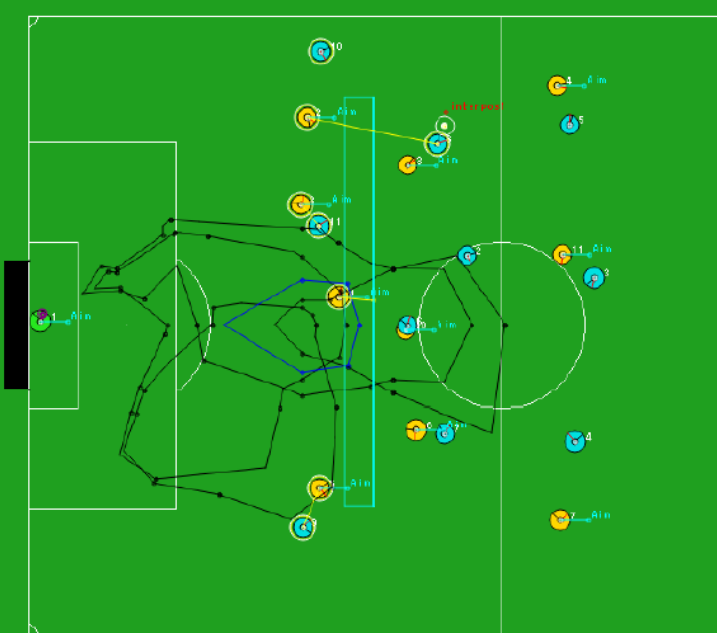
\includegraphics[scale=0.45]{images/wrightEagle_defensenet.png}
    \caption{WrightEagle's defensive net. The blue area represents the area to be defended and the blacks, all calculated areas. Image from \cite{wrighteagle2014}.}
    \label{fig:defensenet}
\end{figure}

\begin{figure}[H]
    \centering
    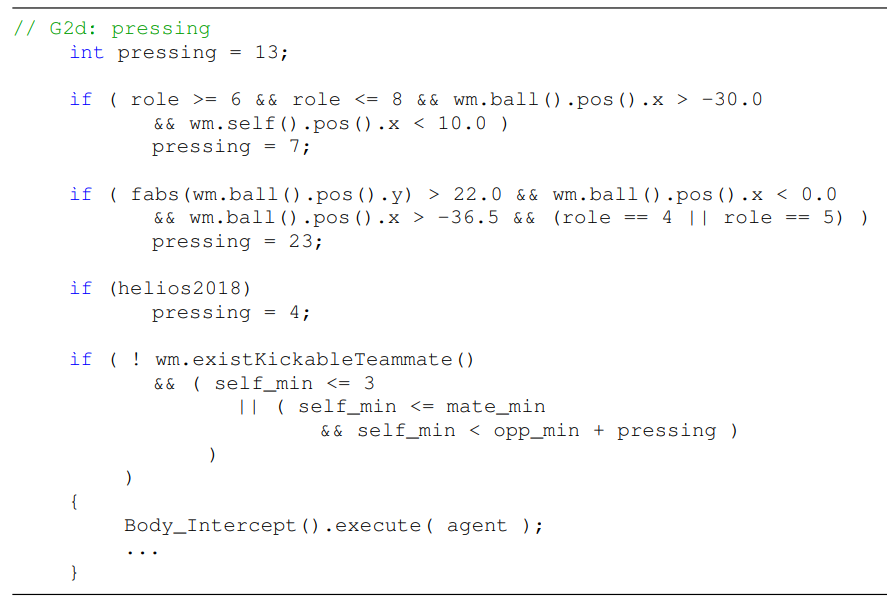
\includegraphics[scale=0.5]{images/gliders_pressing.png}
    \caption{Gliders' piece of code showing the fine tuning of pressing variable. Image from \cite{glidersv1}.}
    \label{fig:gliderscode}
\end{figure}

\section{Reinforcement Learning Agents}\label{section:RLAgents}
In this section we show some algorithms that introduced Reinforcement Learning into the SS2D. All teams here mentioned had a great performance in their years of competition.

\subsection{Brainstormers2d}
The pilot of Reinforcement and Deep Reinforcement Learning was Brainstormers2d. Since 2002 they invest in RL algorithms (\cite{brainstormers2002}) but here we mention only the techniques that gave them the first place in the competition: Intercept ball with RL and the NeuroHassle approach.
\subsubsection{Intercept Ball Task}
\cite{brainstormersIntercept} formalized their technique as a Markov Decision Process, \cite{bertsekas1996neuro}, where the State space was represented by the ball's velocity X and Y directions, agent's velocity X and Y directions, the distance between the agent and the ball and the relative angle between ball and agent. The actions available to the agent were turn and dash commands. They discretized the Environment Space into a grid of \num{6e5} cells. They also considered a noise-free environment to do the experiments.

As \cite{brainstormersIntercept} say, the technique outperformed their previous NI'02 Intercept Model and takes only one more cycle to intercept the ball then the Model Based algorithm described in the paper.

\subsubsection{The NeuroHassle Approach}
Brainstormers did a disruptive job introducing Neural Reinforcement Learning in the Soccer Simulation 2D league in 2006. \cite{neurohassle} technique (it was develop in 2006 but the paper was only published in 2009) shows that a well modeled reinforcement learning system can outperform a deterministic one.
They restricted their state space into a 9 dimensions one considering:
\begin{itemize}
    \item Distance d between defender and the attacker
    \item Velocity (v$_x$ and v$_y$ component) defender
    \item Absolute value of the attacker’s velocity
    \item Position (b$_x$ and b$_y$ component) of the ball
    \item Defender’s body angle relative to the attacker’s position
    \item Attacker’s body angle relative to his direction towards the goal
    \item Value of the angle $\gamma = \angle GAD$ with G as position of the goal, A as position of the attacker, and D as the position of the defender
\end{itemize}
They put as actions a discretized space of 76 dimensions where the first 40 were the dash command  varying the power from -100 to 100 with a 5 step and the last 36 were turn command varying the angle from -180 to 180 with a 10 degree step.

To specialize the agent, they created a set of \textit{training situations} $S$ ($|S|=5000$ described in Figure \ref{fig:neurohassleTS} and defined four \textit{training regions} shown in Figure \ref{fig:neurohassleTR}.

\begin{figure}[H]
    \centering
    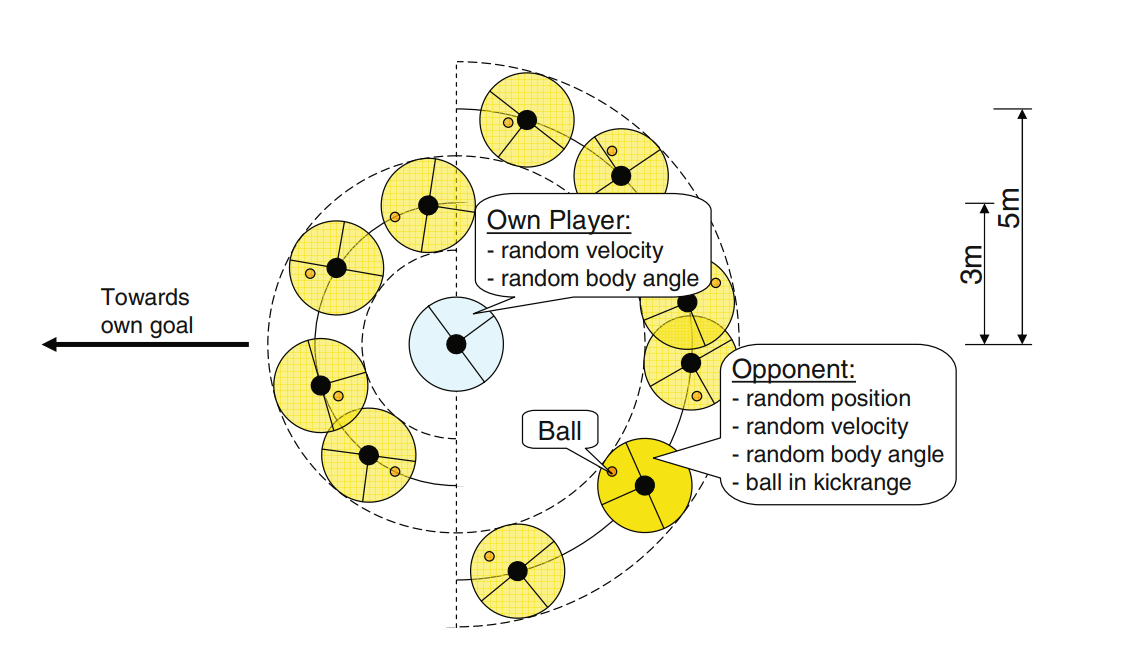
\includegraphics[scale=0.25]{images/neurohassleTS.png}
    \caption{Neurohassle's \textit{training situations}. Image from \cite{neurohassle}.}
    \label{fig:neurohassleTS}
\end{figure}

\begin{figure}[H]
    \centering
    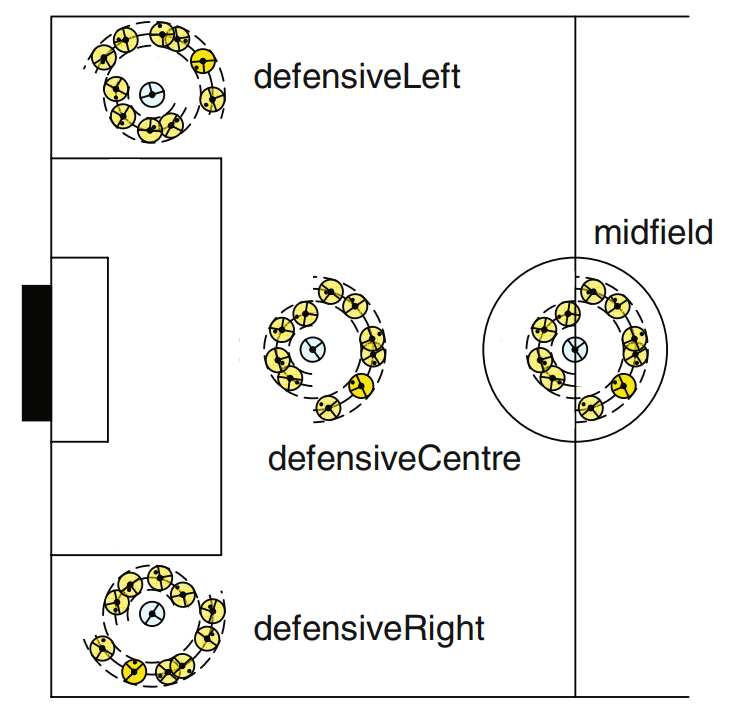
\includegraphics[scale=0.25]{images/neurohassleTR.png}
    \caption{Neurohassle's \textit{training regions}. Image from \cite{neurohassle}.}
    \label{fig:neurohassleTR}
\end{figure}

They did a simple reward function:
\begin{itemize}
    \item For each step without success: small negative reward 
    \item Failure: Large negative reward
    \item Success: Large positive reward
\end{itemize}

The Temporal Difference (TD) loss was calculated as follows:
\begin{gather*}
\label{eq1}
V(s_k) = (1-\alpha)*V(s_k) + \alpha*ret(s_k)
\\
ret(s_k) = \sum_{j=k}^{N} r(s_k, \pi(s_k))
\end{gather*}
Where $V(s_k)$ means the state value function, $ret(s_k)$ the summed rewards following state $s_k$ and $\alpha$ the learning rate. They employed a multi-layer perceptron (MLP) neural networks \cite{mlp} with a 9:18:1-topology to train the agent. See the results on Figure \ref{fig:neurohassleR1} and Figure \ref{fig:neurohassleR2}.

\begin{figure}[H]
    \centering
    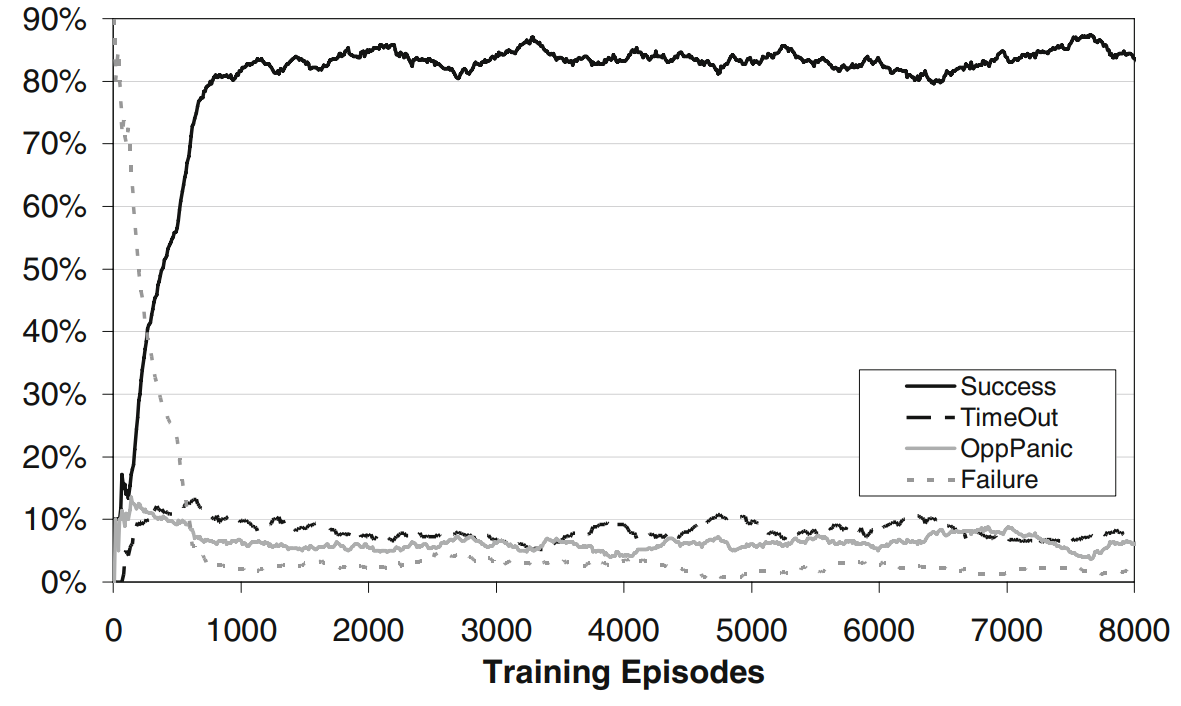
\includegraphics[scale=0.25]{images/neurohassleR1.png}
    \caption{Example of Learning Curve for Learning to Hassle. Image from \cite{neurohassle}.}
    \label{fig:neurohassleR1}
\end{figure}

\begin{figure}[H]
    \centering
    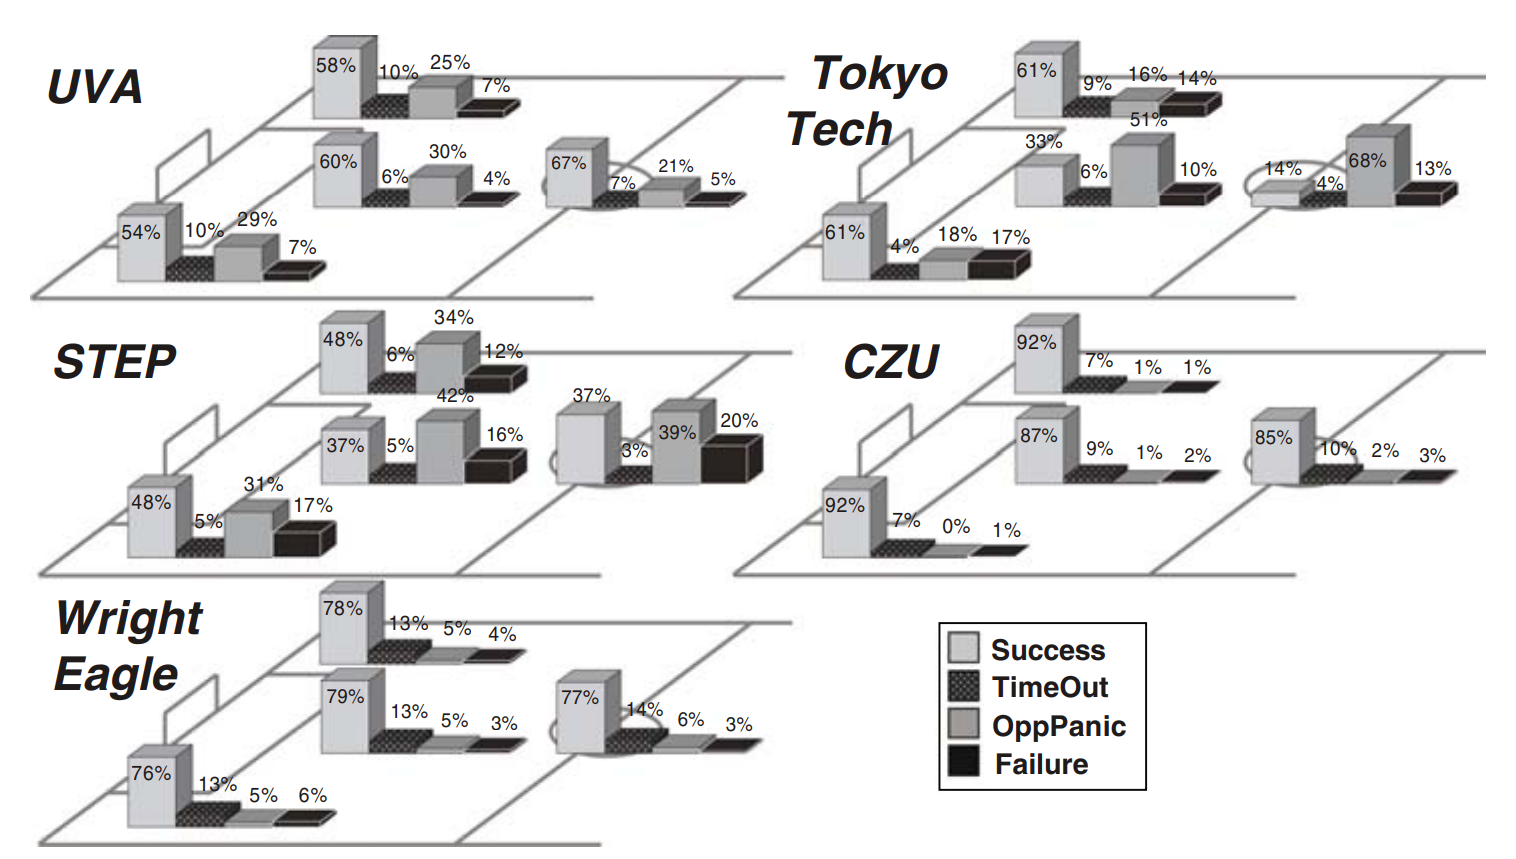
\includegraphics[scale=0.25]{images/neurohassleR2.png}
    \caption{\textit{Training regions} analysis for some teams from RoboCup2006. Image from \cite{neurohassle}.}
    \label{fig:neurohassleR2}
\end{figure}

\subsection{Cyrus2019}
\cite{cyrus} did an interesting job with a single agent cooperating with the goalie against an attacker. They did not specified the space features that they used, but they did tell us about \cite{hfo} environment, so we assumed that they used the high level state features from HFO. The actions they chose were block (\cite{cyrus2014}, a Cyrus' implementation of \cite{marlik2011}'s  Marlik block), intercept ball, cooperation with goalie (the defender ) and move (execute the movement according to the formation file). See Figure \ref{fig:cyrus_block}, \ref{fig:cyrus_intercept}, \ref{fig:cyrus_gassist} for the high level actions. 

\begin{figure}[H]
    \centering
    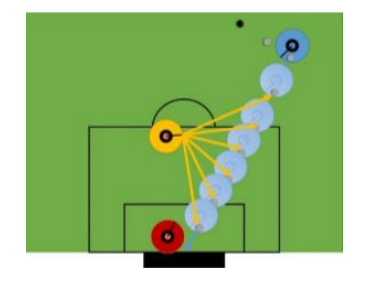
\includegraphics[scale=0.5]{images/cyrus_block.png}
    \caption{Cyrus' Block movement. Image from \cite{cyrus}.}
    \label{fig:cyrus_block}
\end{figure}

\begin{figure}[H]
    \centering
    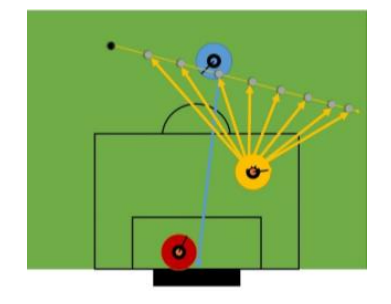
\includegraphics[scale=0.5]{images/cyrus_intercept.png}
    \caption{Intercept movement. Image from \cite{cyrus}.}
    \label{fig:cyrus_intercept}
\end{figure}

\begin{figure}[H]
    \centering
    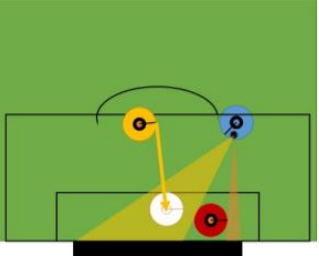
\includegraphics[scale=0.5]{images/cyrus_gassist.png}
    \caption{Cyrus' Goalie Assistant movement. Image from \cite{cyrus}.}
    \label{fig:cyrus_gassist}
\end{figure}

The reward modeling is described in Figure \ref{fig:cyrus_rewards}. They used a Deep Deterministic Policy Gradient (\cite{DDPG}) to train the agent with the TD function explained in Section \ref{section:ddpg}. The results are shown in Figure \ref{fig:cyrus_results}
\begin{figure}[H]
    \centering
    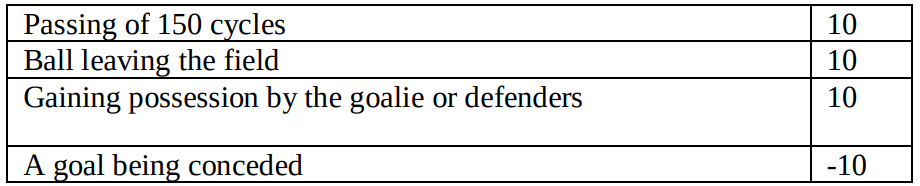
\includegraphics[scale=0.5]{images/cyrus_rewards.png}
    \caption{Cyrus' reward model. Image from \cite{cyrus}.}
    \label{fig:cyrus_rewards}
\end{figure}

\begin{figure}[H]
    \centering
    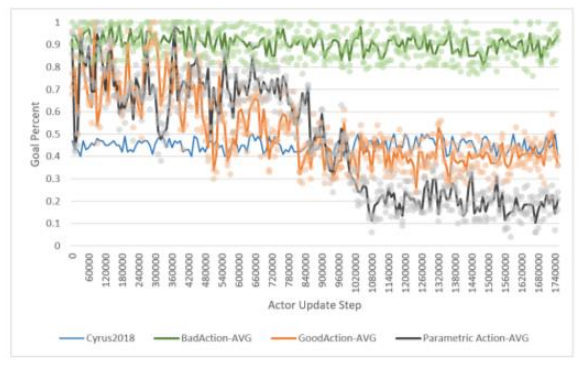
\includegraphics[scale=0.5]{images/cyrus_results.png}
    \caption{Cyrus' DDPG results. The best result is choosing a action and then CYRUS2018 (\cite{cyrus2018}) doing that action. Image from \cite{cyrus}.}
    \label{fig:cyrus_results}
\end{figure}
\chapter{Environment}\label{chapter:environment}

The Half Field Offensive (HFO), \cite{hfo}, is an interface environment designed specifically to train SARSA (state, action, reward, next state, next action) agents based on the usual OpenAI environments. See figure \ref{images/HFO_diagram.png}. It provides 2 spaces of states and 3 spaces of actions:
\begin{itemize}
    \item Low-Level Features and Actions- Uses raw features from Sim2d server and provides raw actions.
    \item Mid-Level Actions - Uses raw features but some complex and chained actions.
    \item High-Level Features and Actions - Uses processed features and only complex or chained actions.
\end{itemize}
We adapted this environment to our problem changing the server's referee, the feature set and the actions that the agents can perform.

\section{Server's Referee}
\begin{itemize}
    \item Half Field Offensive's referee restricts all agents on the right side of the field. Our problem is more complex due to defending on opponent's side as well. Our referee covers the whole field.
    \item Given two areas O and T, opponents spawns randomly on O and the same for teammates on T. We need a spawn similar to a real attack situation in Soccer Simulation 2D. For the defender team We fixed specifics X axis for types of agent and randomizes the Y axis. The midfielders starts in front of the defenders. For the attacking team, is the same logic for attackers and midfielders. We decided to do not randomize the Y axis and fix it on 0 for all attackers.   
    \item The ball always starts near the midfielders of the attacking team in our environment. Doing so, We simulate a counterattack of the opponent.
\end{itemize}

\section{Feature Set}
HFO's high-level features set returns many features that is not relevant for our problem, such as opening angle to opponent's goal or pass opening angle to a teammate. We decided to remove those variables for the models understand more easier what to do. Another change was in the normalization of the features. The original environment returned normalized features in relation due to the half field problem. Once our problem is more comprehensive and the agents are in the same space and the features are strict, We maintained the without normalization. 

Let $T$ denote the number of teammates in game and $O$ the
number of opponents. There are a total of $11 + 3T + 2O + 1$ high-level
features in our environment.

\begin{enumerate}[noitemsep]
\setcounter{enumi}{-1}
\item{\textbf{X position} - The agent’s x-position on the field.}
\item{\textbf{Y position} - The agent’s y-position on the field.}
\item{\textbf{Orientation} - The global direction that the agent is facing.}
\item{\textbf{Ball X} - The ball's x-position on the field.}
\item{\textbf{Ball Y} - The ball's y-position on the field.}
\item{\textbf{Able to Kick} - Boolean indicating if the agent can kick the ball.}
\item{\textbf{Goal Center Proximity} - Agent's proximity to the center of the goal.}
\item{\textbf{Goal Center Angle} - Angle from the agent to the center of the goal.}
\item{\textbf{Proximity to Opponent} - If an opponent is present,
  proximity to the closest opponent. Invalid if there are no
  opponents.}
\item{\textbf{Formation X position} - Agent’s x-position according to team's formation.}
\item{\textbf{Formation Y position} - Agent’s y-position according to team's formation.}
\item [$T$] {\textbf{Proximity from Teammate i to Opponent} - For each
  teammate i: the proximity from the teammate to the closest
  opponent. This feature is invalid if there are no opponents or if
  teammates are present but not detected.}
\item [$2T$] {\textbf{X, Y of Teammates} - For each teammate: the x-position, y-position.}
\item [$2O$] {\textbf{X, Y of Opponents} - For each opponent: the x-position, y-position.}
\item [$+1$] {\textbf{Interceptable} - Whether the agent can intercept the ball or
 not.}
\end{enumerate}

\section{Actions}
Based on \cite{cyrus}, We chose four actions:
\begin{enumerate}
    \item Move: Performs the basic move, going to the position according to the formation file.
    \item Go to ball: Performs an interception move, tackling the opponent when it can.
    \item Block: Blocks a shoot or a pass from an opponent to another.
    \item Defend Goal: Blocks a shoot at the same line of the goalkeeper.
\end{enumerate}

Once the action "Catch" does not fit in our problem yet, We decided to exchange it for Block. We used the algorithm of \cite{cyrus2014}.
% \chapter{Experiments and Results}\label{chapter:results}
\section{Experiments}\label{section:exp}
For the experiments, we used, for the first 100K training episodes of the three techniques, Helios2013's goalie and Helios2013's offensive and for 10K we changed the goalie to RoboCIn2019's. We used \cite{dqn}'s technique to stack 32 states, therefore a state of shape [32x1x16]. The Networks' and memory's parameters is in Figure \ref{fig:hyperparams}. For DQN and DDQN we used the $\epsilon$-greedy technique with $\epsilon$'s maximum at 1.0 and minimum at 0.01. For DDPG we added a noise of 0.1 in the action. The full code is available in \url{https://github.com/goncamateus/graduationMgm}.

The Neural Network's topology were (all using Rectified Linear Unit activation function \cite{relu}):
\begin{itemize}
    \item Deep Q Networks: 512:128:256:4.
    \item Duelling Double Deep Q Networks: 
    
    Advantage - [512:128:128:4]; Value - [512:128:128:1].
    \item Deep Deterministic Policy Gradient: 
    
    Actor - [512:256:128] with output of shape [4x1]; Critic - [512:256:128:1].
\end{itemize}


\begin{figure}
    \centering
    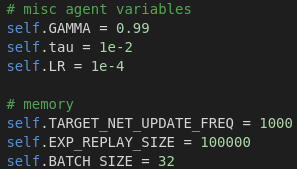
\includegraphics[scale=0.6]{images/hyperparams.png}
    \caption{Neural Networks' and Memory's parameters.}
    \label{fig:hyperparams}
\end{figure}

\section{Results}
In this section we show the graphs and tables of training and tests. As said in Section \ref{section:exp}, the training was 100K episodes with Helios2013's goalie and 10K with RoboCIn2019's goalie. The whole training against Helios2013's attacker.
\subsection{Training}
During the training we could see some interesting behaviours of each learning algorithm. The DQN agent turned out to be the most aggressive agent. Before episode 10K, it started to chase the attacker due to Intercept action. As there is no fault in our domain, the Network found this strategy but it is not the best thing to be done during a real game. Figure \ref{fig:dqnres} shows it's performance with rewards.
\begin{figure}[H]
    \centering
    \subfloat{{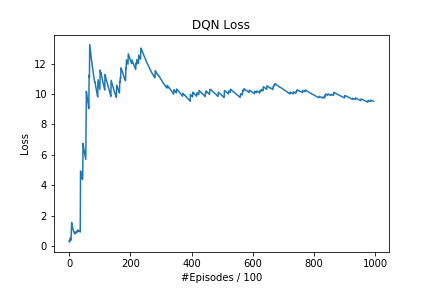
\includegraphics[scale=0.45]{images/dqn_loss.png}}}%
    \qquad
    \subfloat{{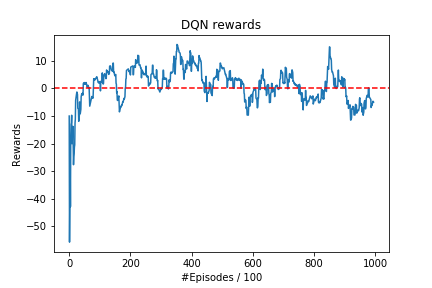
\includegraphics[scale=0.45]{images/dqn_rewards.png}}}%
    \qquad
        \caption{Deep Q Network results. Loss convergence and Rewards in function of number of episodes.}
    \label{fig:dqnres}
\end{figure}

The DDPG agent found a policy very similar to RoboCIn2019's defender but a bit more aggressive. The agent blocks the shoot of the attacker most of time but intercept in the right gap of the attacker. Sometimes the episode takes too long due to the attacker's incapability to decide what to do, that would lead to a fault in real game and the defender would win the ball. Figure \ref{fig:ddpgres} shows the performance of the agent. As we can  see in the Actor Loss, sometime before the episode 20K it found that policy and converged to it.

\begin{figure}[H]
    \centering
    \subfloat{{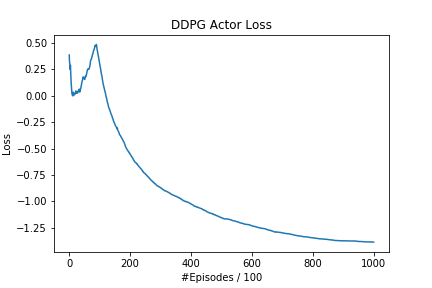
\includegraphics[scale=0.45]{images/ddpg_actor_loss.png}}}%
    \qquad
    \subfloat{{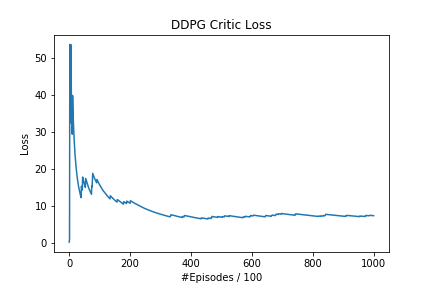
\includegraphics[scale=0.45]{images/ddpg_critic_loss.png}}}%
    \qquad
    \subfloat{{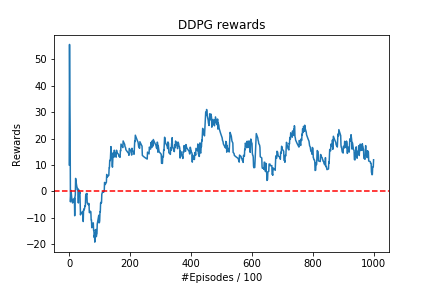
\includegraphics[scale=0.6]{images/ddpg_rewards.png}}}%
    \qquad
    \caption{Deep Deterministic Policy Gradient results. Loss convergence of Actor and Critic networks and Rewards in function of number of episodes.}
    \label{fig:ddpgres}
\end{figure}

The DDQN agent took an intermediate behaviour. Sometimes it acted as DQN's agent but most of time it acted just like DDPG's. The episodes that it acted too aggressive, the attacker shoots to the goal and scores, most of time. Figure \ref{fig:ddqnres} shows the performance of the agent.

\begin{figure}[H]
    \centering
    \subfloat{{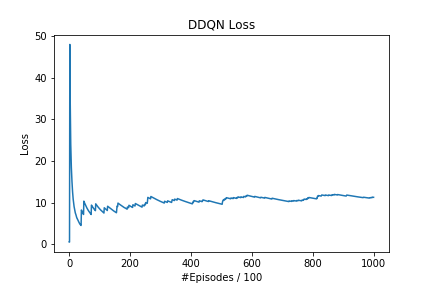
\includegraphics[scale=0.45]{images/ddqn_loss.png}}}%
    \qquad
    \subfloat{{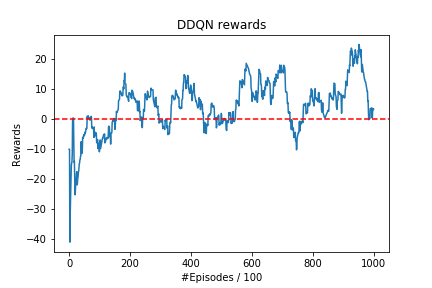
\includegraphics[scale=0.45]{images/ddqn_rewards.png}}}%
    \qquad
        \caption{Duelling Double Deep Q Network results. Loss convergence and Rewards in function of number of episodes.}
    \label{fig:ddqnres}
\end{figure}




\subsection{Tests}
To test, we wanted to compare with the Helios2013 and RoboCIn2019. Helios2013 was chosen because HFO already had support for the team. RoboCIn2019 was chosen because we want to put the best agent in the team. We tested with both attackers and both goalies for 3000 episodes each combination. Table \ref{tab:result_base_line} shows the baseline with Helios2013's and RoboCIn2019's agents. Tables \ref{tab:helios_result} and \ref{tab:rc_result} show the results of the DRL agents with the cooperating with the deterministic goalies against each attacker.

\begin{table}[H]
\begin{center}
\begin{tabular}{|c|c|c|}
\hline

                   & Helios2013 & RoboCIn2019 \\ \hline
Helios2013         & 77,5\%     & 77.4\%      \\ \hline
RoboCIn2019        & 71\%       & 53.3\%      \\ \hline
    \end{tabular}
\end{center}
\caption{Result baseline. Rows are the defenders and Columns are the attackers of each original team. Percentage of successful defenses for 3000 episodes.}
\label{tab:result_base_line}
\end{table}

\begin{table}[H]
\begin{center}
\begin{tabular}{|c|c|c|}
\hline
                   & Helios2013 & RoboCIn2019 \\ \hline
DQN 110k training  & 63\%     & 76.2\%        \\ \hline
DDQN 110k training & 75.1\%       & 72.4\%      \\ \hline
DDPG 110k training & 82.1\%     & 95\%      \\ \hline
\end{tabular}
\end{center}
\caption{Tests for 3000 episodes. Rows are the DRL defenders with Helios2013's goalie and Columns are the attackers. Percentage of successful defenses for 3000 episodes.}
\label{tab:helios_result}
\end{table}


\begin{table}[H]
\begin{center}
\begin{tabular}{|c|c|c|}
\hline
                   & Helios2013 & RoboCIn2019 \\ \hline
DQN 110k training  & 51.3\%     & 64.2\%        \\ \hline
DDQN 110k training & 62.9\%     & 83.6\%      \\ \hline
DDPG 110k training & 70\%     & 86.7\%      \\ \hline
\end{tabular}
\end{center}
\caption{Tests for 3000 episodes. Rows are the DRL defenders with RoboCIn2019's goalie and Columns are the attackers. Percentage of successful defenses for 3000 episodes.}
\label{tab:rc_result}
\end{table}
% \chapter{Conclusion}\label{chapter:conclusion}

The Defense Line is one of the most important task in the Soccer Simulation 2D league. There are many techniques implemented by other teams using deterministic policies that has a great performance. These algorithms came through deep studies in human behaviours in real soccer based on timing of intercept, positioning and blocking passes.

The main problem of those policies is that it is predictable therefore there is a way to break that line. Our work's main intent is to create unpredictable agent to help the goalie and do not receive goals. This work compares 3 Deep Reinforcement Learning algorithms with 2 deterministic teams with great rate of defenses in the SS2D.

We can conclude that DRL has a great potential of applicability in Soccer Simulation 2D due to it's elasticity to learn about the opponent and teammates. We can see in Tables \ref{tab:helios_result} and \ref{tab:rc_result} that the agent has to learn more about RoboCIn2019's goalie than the Helios2013's. DDPG had a great performance in our experiments performing a great percentage of defenses, being better to use rather than the deterministic teams. Also DQN and DDQN had a good performance but stays behind the deterministic algorithms. Based on the results, probably a more specific training for each team will lead to a better performance of each algorithm.


% Uncomment to proposal
% \chapter{Introduction}
A liga de Simulação de Futebol 2D da \cite{robocup} (Sim2d) é uma das mais antigas da competição, tendo início em 1996. As técnicas mais usadas nos 5 melhores times da liga são Aprendizagem Supervisionada e Algorítmos determinísticos. Pesquisas recentes  tem mostrado que usar Aprendizagem Profunda por Reforço (APR) para treinar agentes autônomos em sistemas multi agentes se obtém uma performance maior. O time CYRUS2019, \cite{cyrus}, fez sua linha defensiva de jogadores usando APR e conquistou o terceiro lugar na RoboCup2019.Este trabalho pretende incluir uma linha de defesa treinada com uma técnica de APR baseado no time CYRUS2019, adpatando o ambiente do \textit{Half Field Offensive} para um ambiente OpenAI GYM, \cite{gym}, e aplicar ao time da equipe \cite{robocin}.

Com o objetivo de vencer o time capeão mundial humano de 2050, a RoboCup tem sido uma grande competição para desenvolver e compartilhar técnicas sobre robótica e agentes autônomos. Entre as ligas, Simulação de Futebol 2D é um dos melhores ambientes para se aplicar algoritmos de aprend
With the goal of beating the human soccer World Champion team in 2050, Robocup has been a great competition to develop and share robotics and autonomous agents techniques. Among the leagues, Soccer Simulation 2D league is a great domain to invest machine learning (ML) algorithms and it is been a challenge as \cite{RoboCupAIChallenge} say. At the very beginning of the league at 1996, the competitors used to implement by their own hands the behaviours of the players. Once it's a simulated league, Machine Learning techniques became natural since there is no mechanic or electronic interference. The German team, Brainstormers was one of the pilots with an approach using Reinforcement Learning (\cite{brainstormers2002}). Since then teams frequently uses Artificial Intelligence algorithms to have unnatural and unpredictable behaviours. 

This work focus on the defense line, specifically in a single intelligent defender cooperating with a hand-coded goalie against a single attacker. As there is more works about the attackers like \cite{passingCrit}, \cite{keepawayRL} and more recent \cite{hausknecht2015deep}, the defense line became attractive to the RoboCIn team.

\cite{deepmind} researchers \cite{dqn} have shown that Deep Q Learning was so effective on Atari games that it outplays human controlled agents. In 2015 Deepmind's AlphaGo agent, \cite{alphago}, won from the European Go Champion Fan Hui and later on 2016 from Lee Sedol, one of the best worldwide. Since then OpenAI and DeepMind has invested a lot of effort on Reinforcement Learning (RL) and Autonomous Agents (AA) systems. Recently \cite{openai5} has become the best agent on \cite{dota2} on 1v1 games and it has a great teamwork performance on 5v5 games winning from most of amateur teams and a few professionals.

Inspired by those recent researches \cite{cyrus} modeled a defensive autonomous agent and it has almost the same efficiency of the champions' Fractals (\cite{glidersv2}, and Helios, \cite{helios2016}, defenses. Based on \cite{cyrus} work we will compare three Deep Reinforcement Learning models, \cite{dqn}, \cite{DDQN}, \cite{DDPG}, applied to an environment very likely to the real Soccer Simulation 2D.

% \chapter{Objectives}
The main objective of this work is to analyze the performance of three DRL algorithms on RoboCup's Simulation 2D environment. Deep Q Network (DQN), \cite{dqn}, Dueling Double Q Network (DDQN), \cite{DDQN}, and Deep Deterministic Policy Gradients (DDPG), \cite{DDPG}, algorithms were chosen to be compared. This choice was based on \cite{cyrus} work which applied DDPG on it's defensive agents.

Before the train and test of the algorithms all the environment has to be set doing the following minors objectives:
\begin{itemize}
    \item Adapt HFO server to our context.
    \item Prepare the environment to be like OpenAI GYM.
    \item Choose the features to use on the NNs.
    \item Creation of dataset.
\end{itemize}
% \chapter{Methodology}
\section{Feature Set}
HFO's high-level features set returns many features that is not relevant for our problem, such as opening angle to opponent's goal or pass opening angle to a teammate. We decided to remove those variables for the models understand more easier what to do. Another change was in the normalization of the features. The original environment returned normalized features in relation due to the half field problem. Once our problem is more comprehensive and the agents are in the same space and the features are strict, We maintained the without normalization. 

Let $T$ denote the number of teammates in game and $O$ the
number of opponents. There are a total of $10 + 3T + 2O + 1$ high-level
features in our environment.

\begin{enumerate}[noitemsep]
\setcounter{enumi}{-1}
\item{\textbf{X position} - The agent’s x-position on the field.}
\item{\textbf{Y position} - The agent’s y-position on the field.}
\item{\textbf{Orientation} - The global direction that the agent is facing.}
\item{\textbf{Ball X} - The ball's x-position on the field.}
\item{\textbf{Ball Y} - The ball's y-position on the field.}
\item{\textbf{Able to Kick} - Boolean indicating if the agent can kick the ball.}
\item{\textbf{Goal Center Proximity} - Agent's proximity to the center of the goal.}
\item{\textbf{Goal Center Angle} - Angle from the agent to the center of the goal.}
\item{\textbf{Proximity to Opponent} - If an opponent is present,
  proximity to the closest opponent. Invalid if there are no
  opponents.}
\item [$T$] {\textbf{Proximity from Teammate i to Opponent} - For each
  teammate i: the proximity from the teammate to the closest
  opponent. This feature is invalid if there are no opponents or if
  teammates are present but not detected.}
\item [$2T$] {\textbf{X, Y of Teammates} - For each teammate: the x-position, y-position.}
\item [$2O$] {\textbf{X, Y of Opponents} - For each opponent: the x-position, y-position.}
\item [$+1$] {\textbf{Interceptable} - Whether the agent can intercept the ball or
 not.}
\end{enumerate}

\section{Actions}
Based on \cite{cyrus}, We chose four actions: 
\begin{enumerate}
    \item Move: Performs the basic move, going to the position according to the formation file.
    \item Go to ball: Performs an interception move, tackling the opponent when it can.
    \item Defend Goal: Goes to the circumcenter position of the triangle goalie position, right or left goal post position and attacker position.
    \item Block: Performs \cite{marlik2011}'s Marlik Block.
\end{enumerate}
% \chapter{Schedule}

\begin{center}
    \begin{table}[htp]
        \begin{tabular}{l|c|c|c|c|c|c|c|c|c|c|c|c|c|c|c|c|}
        \cline{2-17}
        & \multicolumn{16}{c|}{\cellcolor[HTML]{C0C0C0}{\color[HTML]{333333} Period}} \\ \hline
        \multicolumn{1}{|l|}{\cellcolor[HTML]{C0C0C0}Activity} & \multicolumn{2}{c|}{August} & \multicolumn{4}{c|}{September} & \multicolumn{4}{c|}{October} & \multicolumn{4}{c|}{November} & \multicolumn{2}{c|}{December} \\ \hline
        \multicolumn{1}{|l|}{Literature Review}                & x            & x            & x      &       &       &       &       &       &       &      &       &       &       &       &               &               \\ \hline
        \multicolumn{1}{|l|}{Algorithm studies}                &              &              & x       & x      & x      & x     &      &      &       &      &       &       &       &       &               &               \\ \hline
        \multicolumn{1}{|l|}{Memories creation}                 &              &              &       &      & x     & x     &       &       &       &      &       &       &       &       &               &               \\
        \hline
        \multicolumn{1}{|l|}{Experiments}                      &              &              &        &       &       & x      & x     & x     & x     & x    &       &       &       &       &               &               \\ \hline
        \multicolumn{1}{|l|}{Evaluation}                       &              &              &        &       &       &       &       &       &      & x    & x     & x      &       &       &               &               \\ \hline
        \multicolumn{1}{|l|}{Writing}                          &              &              &        &       &       &       &       &       &       & x    & x     & x     & x     & x     & x             &               \\ \hline
        \multicolumn{1}{|l|}{Presentation preparation}         &              &              &        &       &       &       &       &       &       &      &       &       &       &       & x             & x             \\ \hline
        \end{tabular}
    \end{table}
\end{center}


% \chapter{Possíveis Avaliadores}
Hansenclever de França Bassani

% \newcommand{\namesigdate}[2][10cm]{%
  \begin{tabular}{@{}p{#1}@{}}
    #2 \\[2\normalbaselineskip] \hrule \\[0pt]
    {\small \begin{center}
    \textit{Tsang Ing Ren (Orientador)}}
    \end{center} \\[2\normalbaselineskip] \hrule \\[0pt]
    {\small \begin{center}\textit{Mateus Gonçalves Machado (Aluno)}\end{center}}
  \end{tabular}
}
\chapter{Assinaturas}
O aluno e o orientador assinam abaixo, comprometendo-se com o desenvolvimento
do projeto descrito neste documento.

\begin{center}
\noindent \namesigdate{} \hfill 
\end{center}

\begin{references}
  \bibliography{references}
\end{references}

% References

% Appendix

% \theappendix
% \begin{center}
    \rowcolors{2}{lightgray!30}{white}
    \begin{longtable}{l|l}
    \caption{%
    List of all features extracted. Class 1 means a lexical feature, Class 2 a semantic feature and 3 a syntactic feature.%
    } \label{tab:long} \\
    Class & Feature \\
	\toprule
    1 & Base name of class package name: accounts \\
    1 & Base name of class package name: io \\
    1 & Base name of class package name: music \\
    1 & Base name of class package name: telephony \\
    1 & Base name of class package name: webkit \\
    1 & Method has parameters \\
    1 & Method is lone getter or setter \\
    2 & Method is part of a ABSTRACT class \\
    2 & Method is part of a FINAL class \\
    2 & Method is part of a PRIVATE class \\
    2 & Method is part of a PROTECTED class \\
    2 & Method is part of a PUBLIC class \\
    2 & Method is part of a STATIC class \\
    2 & Method is part of an anonymous class \\
    2 & Method is part of class android.app.Activity \\
    2 & Method is part of class android.app.BroadcastReceiver \\
    2 & Method is part of class android.app.ContentProvider \\
    2 & Method is part of class android.app.Service \\
    2 & Method is part of class android.content.ContentResolver \\
    2 & Method is part of class android.content.Context \\
    2 & Method is part of class that contains the name com.google.common.io \\
    2 & Method is part of class that contains the name java.io. \\
    2 & Method is part of class that ends with Context \\
    2 & Method is part of class that ends with Factory \\
    2 & Method is part of class that ends with Handler \\
    2 & Method is part of class that ends with Loader \\
    2 & Method is part of class that ends with Manager \\
    2 & Method is part of class that ends with Service \\
    2 & Method is part of class that ends with View \\
    2 & Method is thread runner \\
    2 & Method modifier is FINAL \\
    3 & Method modifier is PROTECTED \\
    2 & Method modifier is PUBLIC \\
    2 & Method modifier is STATIC \\
    1 & Method name ends with Messenger \\
    1 & Method name starts with <init> \\
    1 & Method name starts with add \\
    1 & Method name starts with apply \\
    1 & Method name starts with bind \\
    1 & Method name starts with clear \\
    1 & Method name starts with close \\
    1 & Method name starts with delete \\
    1 & Method name starts with disable \\
    1 & Method name starts with dispatch \\
    1 & Method name starts with do \\
    1 & Method name starts with dump \\
    1 & Method name starts with enable \\
    1 & Method name starts with finish \\
    1 & Method name starts with get \\
    1 & Method name starts with handle \\
    1 & Method name starts with insert \\
    1 & Method name starts with is \\
    1 & Method name starts with load \\
    1 & Method name starts with note \\
    1 & Method name starts with notify \\
    1 & Method name starts with onClick \\
    1 & Method name starts with open \\
    1 & Method name starts with perform \\
    1 & Method name starts with process \\
    1 & Method name starts with put \\
    1 & Method name starts with query \\
    1 & Method name starts with register \\
    1 & Method name starts with release \\
    1 & Method name starts with remove \\
    1 & Method name starts with request \\
    1 & Method name starts with restore \\
    1 & Method name starts with run \\
    1 & Method name starts with send \\
    1 & Method name starts with set \\
    1 & Method name starts with start \\
    1 & Method name starts with supply \\
    1 & Method name starts with toggle \\
    1 & Method name starts with unregister \\
    1 & Method name starts with update \\
    2 & Method returns constant \\
    2 & Method starts with on and has void/bool return type \\
    2 & Parameter is interface \\
    3 & Parameter to abstract sink \\
    3 & Parameter to sink method adjust \\
    3 & Parameter to sink method bind \\
    3 & Parameter to sink method broadcast \\
    3 & Parameter to sink method clear \\
    3 & Parameter to sink method com.android.internal.telephony.CommandsInterface \\
    3 & Parameter to sink method connect \\
    3 & Parameter to sink method create \\
    3 & Parameter to sink method delete \\
    3 & Parameter to sink method dial \\
    3 & Parameter to sink method disable \\
    3 & Parameter to sink method dispatch \\
    3 & Parameter to sink method dump \\
    3 & Parameter to sink method enable \\
    3 & Parameter to sink method enqueue \\
    3 & Parameter to sink method insert \\
    3 & Parameter to sink method notify \\
    3 & Parameter to sink method onCreate \\
    3 & Parameter to sink method perform \\
    3 & Parameter to sink method println \\
    3 & Parameter to sink method put \\
    3 & Parameter to sink method remove \\
    3 & Parameter to sink method replace \\
    3 & Parameter to sink method restore \\
    3 & Parameter to sink method save \\
    3 & Parameter to sink method send \\
    3 & Parameter to sink method set \\
    3 & Parameter to sink method setup \\
    3 & Parameter to sink method show \\
    3 & Parameter to sink method start \\
    3 & Parameter to sink method sync \\
    3 & Parameter to sink method transact \\
    3 & Parameter to sink method update \\
    3 & Parameter to sink method write \\
    2 & Parameter type contains android.content.contentresolver \\
    2 & Parameter type contains android.content.context \\
    2 & Parameter type contains android.content.intent \\
    2 & Parameter type contains android.database.cursor \\
    2 & Parameter type contains android.filterfw.core.filtercontext \\
    2 & Parameter type contains android.net.uri \\
    2 & Parameter type contains com.android.inputmethod.keyboard.key \\
    2 & Parameter type contains com.google.common.io \\
    2 & Parameter type contains event \\
    2 & Parameter type contains java.io. \\
    2 & Parameter type contains java.io.filedescriptor \\
    2 & Parameter type contains java.lang.string \\
    2 & Parameter type contains observer \\
    2 & Parameter type contains writer \\
    1 & Permission name is ACCESS COARSE LOCATION \\
    1 & Permission name is ACCESS FINE LOCATION \\
    1 & Permission name is ACCESS LOCATION EXTRA COMMANDS \\
    1 & Permission name is ACCESS NETWORK STATE \\
    1 & Permission name is ACCESS WIFI STATE \\
    1 & Permission name is ADD VOICEMAIL \\
    1 & Permission name is AUTHENTICATE ACCOUNTS \\
    1 & Permission name is BACKUP \\
    1 & Permission name is BLUETOOTH \\
    1 & Permission name is BLUETOOTH ADMIN \\
    1 & Permission name is BROADCAST STICKY \\
    1 & Permission name is CALL PHONE \\
    1 & Permission name is CALL PRIVILEGED \\
    1 & Permission name is CAMERA \\
    1 & Permission name is CHANGE CONFIGURATION \\
    1 & Permission name is CHANGE NETWORK STATE \\
    1 & Permission name is CHANGE WIFI STATE \\
    1 & Permission name is CLEAR APP USER DATA \\
    1 & Permission name is DEVICE POWER \\
    1 & Permission name is DISABLE KEYGUARD \\
    1 & Permission name is DUMP \\
    1 & Permission name is GET ACCOUNTS \\
    1 & Permission name is GET TASKS \\
    1 & Permission name is GLOBAL SEARCH \\
    1 & Permission name is INTERNET \\
    1 & Permission name is KILL BACKGROUND PROCESSES \\
    1 & Permission name is MANAGE ACCOUNTS \\
    1 & Permission name is MANAGE APP TOKENS \\
    1 & Permission name is MODIFY AUDIO SETTINGS \\
    1 & Permission name is MODIFY PHONE STATE \\
    1 & Permission name is MOUNT UNMOUNT FILESYSTEMS \\
    1 & Permission name is NFC \\
    1 & Permission name is READ CALENDAR \\
    1 & Permission name is READ CALL LOG \\
    1 & Permission name is READ CONTACTS \\
    1 & Permission name is READ EXTERNAL STORAGE \\
    1 & Permission name is READ HISTORY BOOKMARKS \\
    1 & Permission name is READ PHONE STATE \\
    1 & Permission name is READ SMS \\
    1 & Permission name is READ SOCIAL STREAM \\
    1 & Permission name is READ SYNC SETTINGS \\
    1 & Permission name is READ SYNC STATS \\
    1 & Permission name is READ USER DICTIONARY \\
    1 & Permission name is REBOOT \\
    1 & Permission name is RECEIVE BOOT COMPLETED \\
    1 & Permission name is RECEIVE SMS \\
    1 & Permission name is RECORD AUDIO \\
    1 & Permission name is RESTART PACKAGES \\
    1 & Permission name is SEND SMS \\
    1 & Permission name is SET DEBUG APP \\
    1 & Permission name is SET TIME ZONE \\
    1 & Permission name is SET WALLPAPER \\
    1 & Permission name is SET WALLPAPER COMPONENT \\
    1 & Permission name is STOP APP SWITCHES \\
    1 & Permission name is SYSTEM ALERT WINDOW \\
    1 & Permission name is UPDATE DEVICE STATS \\
    1 & Permission name is USE CREDENTIALS \\
    1 & Permission name is USE SIP \\
    1 & Permission name is VIBRATE \\
    1 & Permission name is WAKE LOCK \\
    1 & Permission name is WRITE CALENDAR \\
    1 & Permission name is WRITE CONTACTS \\
    1 & Permission name is WRITE EXTERNAL STORAGE \\
    1 & Permission name is WRITE HISTORY BOOKMARKS \\
    1 & Permission name is WRITE SETTINGS \\
    1 & Permission name is WRITE SMS \\
    1 & Permission name is WRITE SOCIAL STREAM \\
    1 & Permission name is WRITE SYNC SETTINGS \\
    1 & Permission name is WRITE USER DICTIONARY \\
    2 & Return type is android.database.Cursor \\
    2 & Return type is android.net.Uri \\
    2 & Return type is android.os.Parcelable \\
    2 & Return type is boolean \\
    2 & Return type is byte[] \\
    2 & Return type is com.android.internal.telephony.Connection \\
    2 & Return type is int \\
    2 & Return type is java.util.List \\
    2 & Return type is java.util.Map \\
    2 & Return type is void \\
    3 & Value from method get to sink method \\
    3 & Value from method parameter to native method \\
    3 & Value from source method create to return \\
    3 & Value from source method get to return \\
    3 & Value from source method is to return \\
    3 & Value from source method obtainMessage to return \\
    3 & Value from source method query to return \\
    3 & Value from source method writeToParcel to return \\
    3 & Method starting with insert invoked \\
    \bottomrule
    \end{longtable}
    \end{center}
    
    \end{document}

\end{document}
